%% Figure 2 (design of Experiment 2) as a separate artwork file.
%% Build: pdflatex -jobname=Figure_2_full Figure_2, then crop the page to the
%% drawing (scripts/34_crop_figure.py) to obtain Figure_2.pdf.
\documentclass[10pt]{article}
\usepackage[T1]{fontenc}
\usepackage{lmodern}
\usepackage[paperwidth=20cm,paperheight=10cm,margin=0.5cm]{geometry}
\usepackage{tikz}
\usetikzlibrary{arrows.meta,positioning,fit,calc}
\pagestyle{empty}
\begin{document}
\noindent
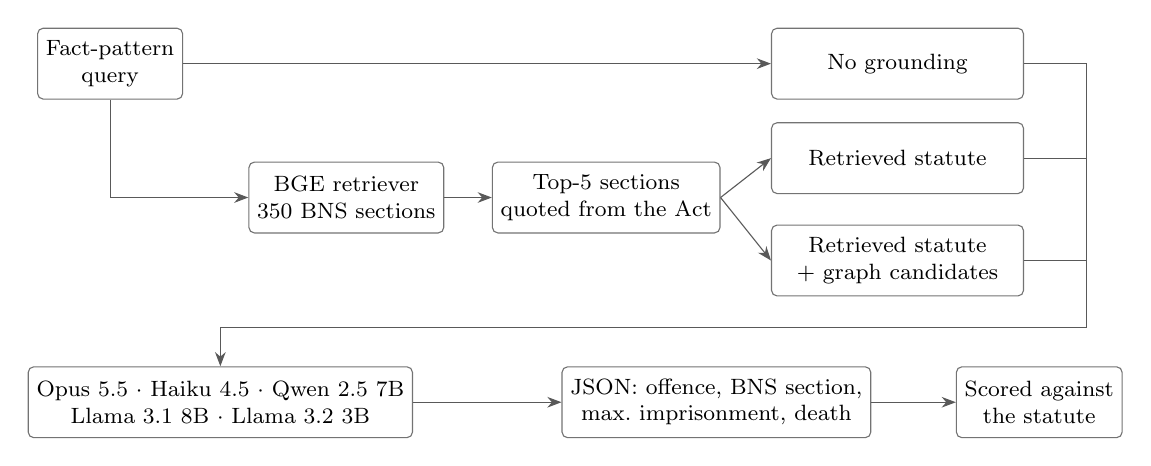
\begin{tikzpicture}[font=\footnotesize,
  box/.style={draw=black!55, rounded corners=2pt, align=center, inner sep=3pt,
              minimum height=9mm, fill=white},
  cond/.style={box, minimum width=32mm},
  arr/.style={-{Stealth[length=1.8mm]}, black!65},
  ln/.style={black!65}]
\node[box]  (q)  at (0.0,  0.6)  {Fact-pattern\\query};
\node[box]  (r)  at (3.0, -1.1)  {BGE retriever\\350 BNS sections};
\node[box]  (t)  at (6.3, -1.1)  {Top-5 sections\\quoted from the Act};
\node[cond] (c1) at (10.0, 0.6)  {No grounding};
\node[cond] (c2) at (10.0,-0.6)  {Retrieved statute};
\node[cond] (c3) at (10.0,-1.9)  {Retrieved statute\\+ graph candidates};
\node[box]  (m)  at (1.4, -3.7)  {Opus 5.5 $\cdot$ Haiku 4.5 $\cdot$ Qwen 2.5 7B\\Llama 3.1 8B $\cdot$ Llama 3.2 3B};
\node[box]  (j)  at (7.7, -3.7)  {JSON: offence, BNS section,\\max.\ imprisonment, death};
\node[box]  (s)  at (11.8,-3.7)  {Scored against\\the statute};
% query to the ungrounded condition, above the retrieval row
\draw[arr] (q.east) -- (c1.west);
% retrieval path
\draw[arr] (q.south) |- (r.west);
\draw[arr] (r) -- (t);
\draw[arr] (t.east) -- (c2.west);
\draw[arr] (t.east) -- (c3.west);
% the three conditions merge on a bus and feed the models
\draw[ln] (c1.east) -- (12.4, 0.6);
\draw[ln] (c2.east) -- (12.4,-0.6);
\draw[ln] (c3.east) -- (12.4,-1.9);
\draw[ln] (12.4,0.6) -- (12.4,-2.75) -- (1.4,-2.75);
\draw[arr] (1.4,-2.75) -- (m.north);
\draw[arr] (m) -- (j);
\draw[arr] (j) -- (s);
\end{tikzpicture}
\end{document}
